\chapter{OFDM in Gnu Radio}
\label{cha:789}
La prima parte del lavoro svolto è consistita nell'implementazione di OFDM nell'ambiente GnuRadio. Il funzionamento di OFDM necessita di vari meccanismi complessi come l'assegnazione di informazioni alle sottoportanti, le correzioni in frequenza, l'equalizzazione e la correzione d'errore come precedentemente spiegato nella parte teorica. Lo svolgimento di queste operazioni sono rese possibili dalla presenza sia di blocchi generici utili ad esempio per la correzione d'errore che di blocchi disponibili specificamente per l'implementazione di OFDM. Per una comunicazione standard OFDM in Gnuradio non è necessaria la scrittura di algoritmi, il lavoro consiste nel collegamento e nella configurazione dei parametri al fine di fare comunicare tutto nella maniera corretta.
La comunicazione è divisa in due parti, una per la trasmissione che ha il compito di generare campioni per il driver dell'usrp-sdr ed una per la ricezione che partendo dai campionamenti effettuati dall'rtl-sdr decodifica le informazioni. Di seguito verranno documentate parte per parte tutte le fasi necessarie.
E' stato scelto di trasferire un file audio in formato wma perchè non effettuando compressioni non viene influenzato dalla mancanza di campionamenti. L'unico problema si verifica eventualmente quando i campioni persi fanno parte della piccola sezione riservata ai metadati. Un pacchetto perso risulterà in circa mezzo millisecondo di audio mancante. La frequenza scelta per la trasmissione è 915Mhz che risulta disponibile per uso civile in Italia \cite{frequenze}, la scelta non ha potuto comprendere 2.4ghz e 5ghz visto che l'Sdr economico utilizzato in ricezione arriva a massimo 2Ghz.
 \section{Trasmettitore}
 La trasmissione è composta da quattro sezioni principali connesse fra loro.
 \begin{itemize}
 	\item \subsection{Formazione pacchetti dal flusso in ingresso}
 	\begin{figure}[h]
 		\centering
 		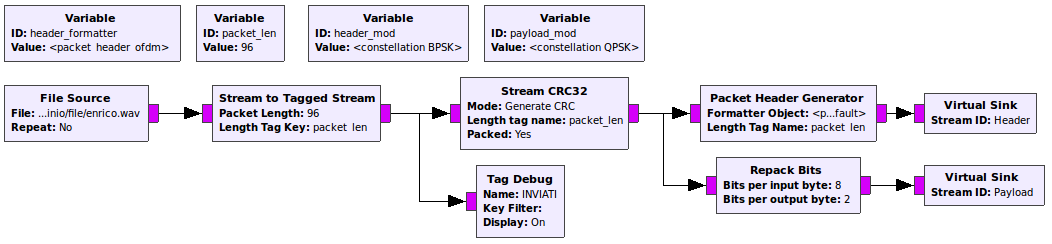
\includegraphics[scale=0.4]{Tx1}
 		\caption{}
 	\end{figure}
 Le informazioni vengono lette da file e fornite dal blocco "File Source" 8bit alla volta, questi byte vengono poi aggregati 96 alla volta tramite l'aggiunta di un tag. A questo punto il blocco "CRC32" appende il codice di controllo per permettere al ricevitore di verificare la presenza di errori. Le informazioni a questo punto vengono processate sia dal blocco "Repack bits" che ha il compito di generare quattro nuovi byte con soli due bit dell'input (la costellazione qpsk permette l'invio di 2 bit alla volta quindi i 6 restanti lasciati a zero e verranno ignorati) che dal blocco "Packet Header generator". Quest'ultimo ha il compito di generare gli header dei pacchetti che permettono al ricevitore di riconoscere l'inizio di un blocco di 96byte+crc di informazione. Gnuradio mette a disposizione degli oggetti "costellation" che contengono informazioni utili relative alle caratteristiche delle costellazioni, ad esempio il numero di bit significativi per la costellazione oppure la mappatura fra bit e punti delle costellazioni (Ad esempio l' oggetto digital.constellation\_qpsk viene utilizzato nel modulo "Repack bits" chiamando la funzione bits\_per\_symbol() che restituisce 2). Le informazioni vengono poi trasferite a due "Virtual Sink" che fungono solamente da collegamento logico verso i "Virtual Source", il loro scopo è quello di rendere la composizione più leggibile.
 	\item \subsection{Codifica informazioni in Simboli}
 	\begin{figure}[h]
 		\centering
 		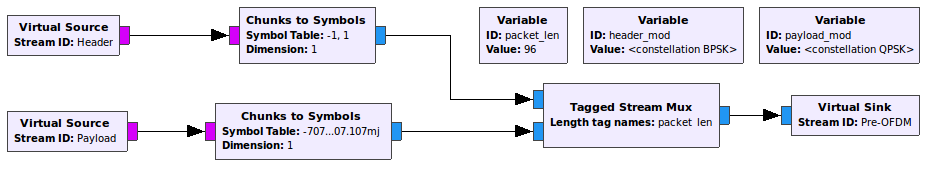
\includegraphics[scale=0.4]{Tx2}
 		\caption{}
 	\end{figure}
 Questa sezione del trasmettitore riceve due flussi dalla precedente contenenti i bit divisi fra header e payload. Il blocchi "Chunks to Symbols" convertono i bit (che ricordiamo sono già nel formato 1 bit significativo per byte per l' header e 2 bit significativi per byte per il payload) in numeri complessi della rispettiva costellazione. La mappatura fra bit significativi e numeri complessi viene fornita dall'oggetto di appoggio disponibile per le varie modulazioni fornito da gnuradio descritto brevemente nel punto precedente chiamando rispettivamente le funzioni payload\_mod.points() e header\_mod.points(). A questo punto è necessario unire in un solo flusso (mantenendo la divisione fedele ai blocchi iniziali) i punti delle costellazioni ottenuti ricalcolando il tag della lunghezza, questo lavoro viene eseguito dal blocco "Tagged Stream Mux".
 	\item \subsection{Allocazione simboli sulle sottoportanti e creazione campioni per l'SDR}
 	\begin{figure}[h]
 		\centering
 		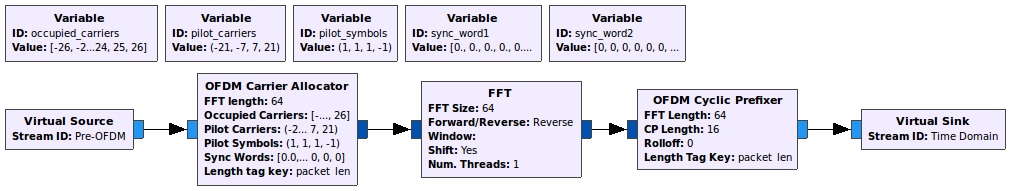
\includegraphics[scale=0.4]{Tx3}
 		\caption{}
 	\end{figure}
 L' obiettivo di questa sezione è quello di allocare sulle sottoportanti di OFDM le informazioni e creare i campioni da spedire nel dominio del tempo. Il blocco "OFDM Carrier Allocator" si occupa di allocare i punti delle costellazioni e i simboli pilota (pilot\_symbols) rispettivamente alle sottoportanti definite come occupied\_carriers e pilot\_carriers. Inoltre aggiunge all'inizio di ogni blocco trasmesso i sync\_words utilizzati dal ricevitore per sincronizzazione ed equalizzazione. L'output rappresenta un simbolo OFDM pronto per essere portato nel dominio del tempo dal blocco  "FFT" che esegue appunto la trasformata di fourier veloce. Il blocco "OFDM Cyclic Prefixer" aggiunge il prefisso ciclico spiegato in precedenza.
 
 	\item \subsection{Passaggio dati all'SDR}
 	\begin{figure}[h]
 		\centering
 		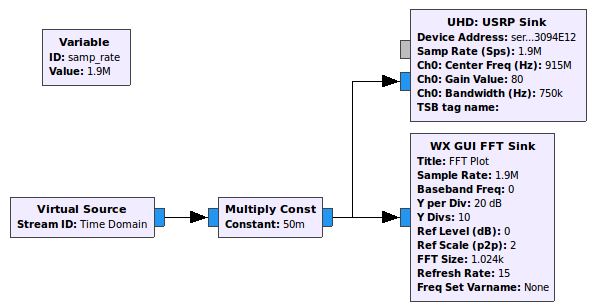
\includegraphics[scale=0.4]{Tx4}
 		\caption{}
 	\end{figure}
 \end{itemize}
L'ultima operazione consiste nel passare il simbolo OFDM al driver dell'SDR configurandolo con i parametri necessari per la trasmissione. Il blocco "WX GUI FFT Sink" serve per avere un feedback sulla trasmissione mostrando un grafico sul dominio delle frequenze (Riportato nella sezione "ortogonalità delle sottoportanti OFDM").
 \section{Ricevitore}
 La ricezione è composta da tre sezioni principali connesse fra loro.
 \begin{itemize}
 	\item \subsection{Ricezione informazioni, sincronizzazione}
 	\begin{figure}[h]
 		\centering
 		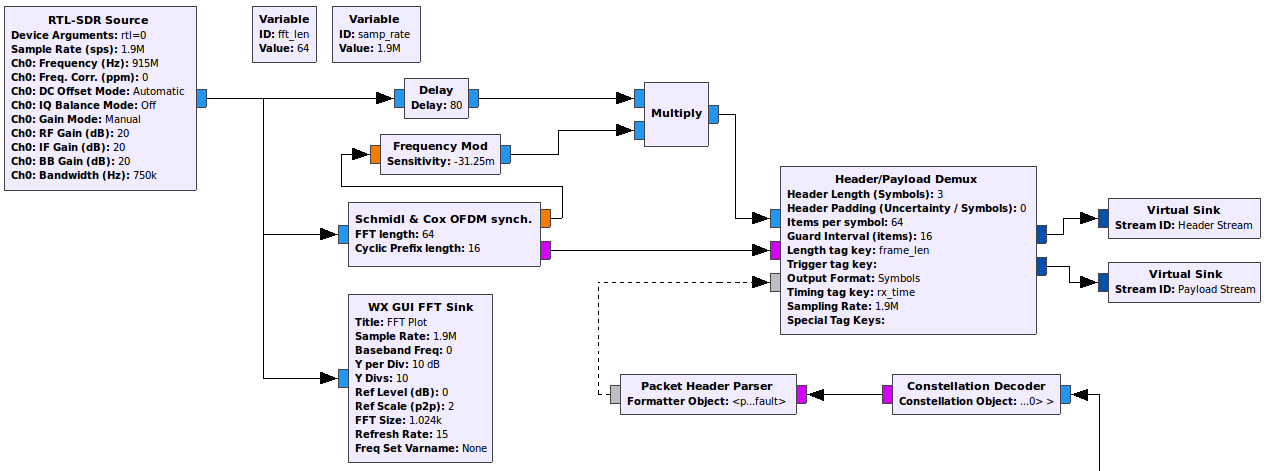
\includegraphics[scale=0.4]{Rx1}
 		\caption{}
 	\end{figure}
 Questa prima sezione del ricevitore ha il compito di leggere i campionamenti forniti dal driver per l'rtl-sdr e ottenere le informazioni nuovamente divise fra header e payload. Il blocco centrale di questa sezione è senzadubbio "Header/payload Demux" che ha proprio questo compito strettamente necessario per poi poter essere analizzati in seguito. I campionamenti sono forniti in forma complessa (I/Q) e rappresentano l'ampiezza del segnale in quell'istante ma anche l' andamento della funzione che lo ha generato. Il processo di ricezione ha inizio quando il blocco "Schmidl \& Cox OFDM sync" individua l'inizio della trasmissione inviando un segnale di comando (trigger) verso il demuxer. Il suo funzionamento è molto complesso e permette assieme al blocco "Frequency mod" la sincronizzazione necessaria per l'inizio della lettura. Il blocco "Header/payload Demux" inoltra sulla prima uscita (Header Stream) i primi 3 simboli OFDM (composti da 64 campioni ognuno) e rimane in attesa fino a che non gli vengono fornite le informazioni contenute nell'header. L'analisi dei campioni contenenti le informazioni sul payload verrà approfondita nella sezione successiva, per ora è importante notare che "Header/payload Demux" riceve queste informazioni sul terzo ingresso. A questo punto il demuxer grazie alle informazioni dell' header può inoltrare il numero corretto di campioni corrispondenti ai simboli OFDM sulla seconda uscita (Payload Stream).
 	\item \subsection{Equalizzazione e ottenimento simboli}
 	\begin{figure}[h]
 		\centering
 		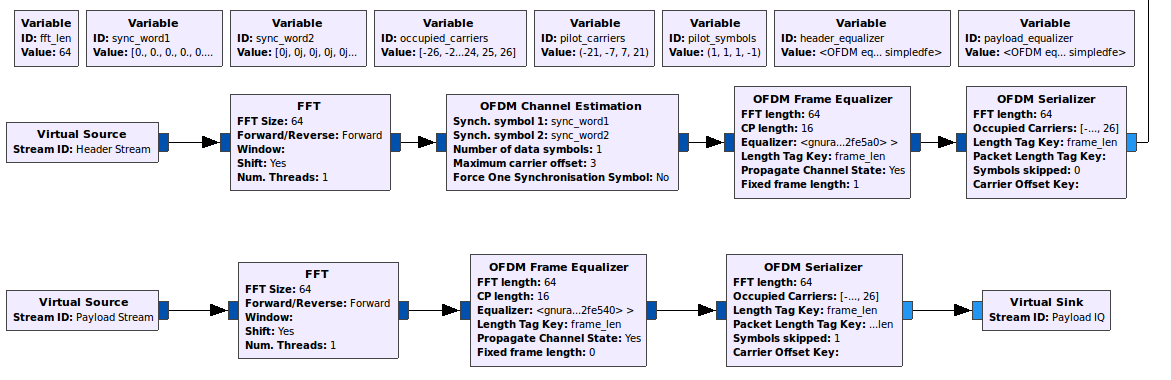
\includegraphics[scale=0.4]{Rx2}
 		\caption{}
 	\end{figure}
 	L' obiettivo di questa sezione è quello di ottenere dai campionamenti ricevuti le costellazioni delle sottoportanti OFDM. La procedura consiste nell' applicazione della trasformata di Fourier veloce per passare al dominio delle frequenze. Nella decodifica dell' header è presente il blocco "Channel Estimator" che sfruttando i primi due sync\_words ha lo scopo di ottenere informazioni di partenza sulle caratteristiche di sfasatura CFO (Carrier Frequancy Offset) e di attenuazione canale. Il blocco successivo "OFDM Frame Equalizer" utilizza queste informazioni per effettuare la prima equalizzazione, le informazioni sulle caratteristiche del canale vengono poi aggiornate alla ricezione di ogni simbolo OFDM grazie ai simboli pilota contenuti nelle apposite sottoportanti. L' ultima operazione della sezione viene svolta dal blocco "OFDM Serializer" e consiste nell'invertire il lavoro svolto dall'allocatore nella fase di trasmissione al fine di ottenere un flusso contente solo i punti delle costellazioni che contengono informazioni in modo ordinato e raggruppati secondo pacchetto di trasmissione (mediante l'aggiunta di un tag). 
 	
 	\item \subsection{Decodifica payload e scrittura file}
 	\begin{figure}[h]
 		\centering
 		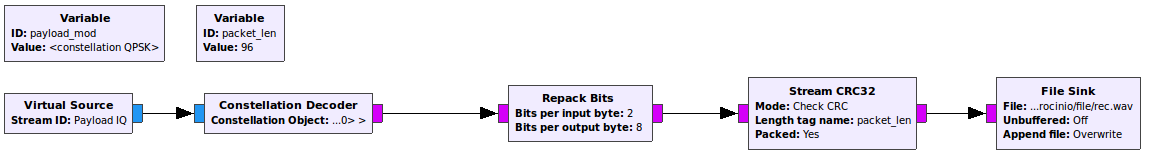
\includegraphics[scale=0.4]{Rx3}
 		\caption{}
 	\end{figure}
 	Il blocco "Constellation Decoder" effettua la decodifica dei numeri complessi ricevuti. Le informazioni ottenute dalla decodifica di una singola costellazione in qpsk sono rappresentabili in 2 bit, è dunque necessario l'utilizzo del blocco "Repack bits" che preleva solo i due bit significativi di quattro decodifiche successive per completare un byte. Sono ancora contenute informazioni relative all'appartenenza ad un blocco coerenti con quelle iniziali in fase di trasmissione, "Stream CRC32" esegue la verifica pacchetto per pacchetto scartandolo se contenente errori. In conclusione il blocco "File Sink" si occupa della scrittura su file completando il processo di ricezione.
 \end{itemize}
\section{Testing}
\subsection{Caratteristiche generali del sistema sotto test}
 Sono stati effettuati alcuni test per osservare il comportamento in un ambiente reale. Le misurazioni sono state effettuate trasferendo un file audio contenente 1.9MB ad una distanza di due metri. La frequenza per la trasmissione è 915Mhz con un bandwidth di 750khz. L'alternativa sarebbe stata 433Mhz ma un breve test non ha rilevato sostanziali differenze nè sulla quantità dei dati ricevuti nè sulle risorse impiegate dai due computer.
 Un altro dato interessante è che la quantità di cpu utilizzata per la parte di trasmissione confrontata con quella per la ricezione è risultata essere il 30\% più onerosa (il confronto è stato fatto rapportando la percentuale di cpu usata sui due computer in relazione al benchmark sul singolo core).
 \subsection{Parametri specifici}
 Nell'eseguire le misurazioni per il grafico 6.1 e 6.2 la trasmissione impiegava 9.2 secondi, il throughput era dunque di 1.6Mb/s con frequenza di campionamento di 1.8Msps.
 La determinazione della qualità del suono ricevuto (G6.1) è stata effettuata facendo ascoltare i vari file ricevuti in maniera non ordinata a due persone distinte chiedendo di giudicarli da 0 a 5 considerando 5 la qualità del file originale e 1 la soglia minima sotto la quale risulta impossibile la comprensione.
 E' possibile osservare l'effetto della perdita dei pacchetti sull' audio ricevuto in Figura 6.8.
 \\I grafici 6.5 e 6.4 sono utili per capire come la frequenza dei campionamenti giochi un ruolo fondamentale nel sistema.
 La sezione blu rappresenta il range dentro il quale si riescono a ricevere informazioni. Per valori di sample-rate minori di 1.7Msps il sistema non è in grado di ricevere informazioni. Questo è dovuto al limite matematico che impone di avere campionamenti in numero almeno doppio rispetto alla larghezza di banda utilizzata.
 Valori superiori di 2Msps non sono raggiungibili con l'SDR-RTL che compromette subito la comunicazione.
 \\Durante l'esecuzione dei test variando il sample-rate è stato notato che superato il 104\% di utilizzo della cpu sul computer in trasmissione avveniva un rallentamento dell'esecuzione del flusso in Gnuradio non generando tutti i campioni, la mia supposizione è che in questa particolare applicazione la divisione del lavoro su più core effettuata automaticamente da Gnuradio si limiti a quel 4\%
 
 
 
  % (decibel non calibrati, sdr con poco range su frequenza e sample rate)
 
 \begin{figure}
 	\centering
 	\begin{minipage}[b]{.45\columnwidth}
 	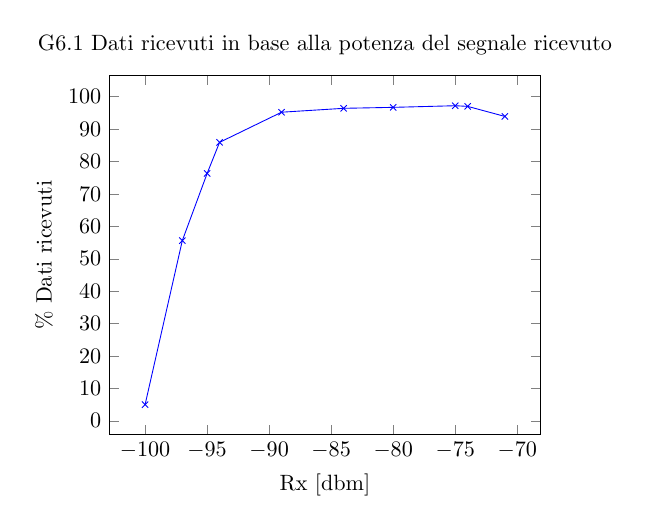
\begin{tikzpicture}[scale=0.8,line width=1pt]
 \begin{axis}[
 ytick={0,10,20,30,40,50,60,70,80,90,100},
 %xtick={0,3.84,5.76,11.52,15.36,23.4},
 %xtick={-110},
 %title = bandwidth rapportato al throughput utente nelle varie TM,
 title =G6.1 Dati ricevuti in base alla potenza del segnale ricevuto,
 grid style=dashed,
 xlabel={Rx [dbm]},
 ylabel={\% Dati ricevuti},
 legend style={at={(0.7,0.02)},anchor=south west}
 ]
 %tm1
 \addplot[
 color=blue,
 mark=x]
 table[x=power,y=BER] {
 	power BER
 	-71 +93.9
 	-74 +97
 	-75 +97.2
 	-80 +96.7
 	-84 +96.4
 	-89 +95.2
 	-94 +85.9
 	-95 +76.3
 	-97 +55.6
 	-100 +5.0
 }; 
 \end{axis}
 \end{tikzpicture}
\end{minipage}
 \centering
 \begin{minipage}[b]{.45\columnwidth}
  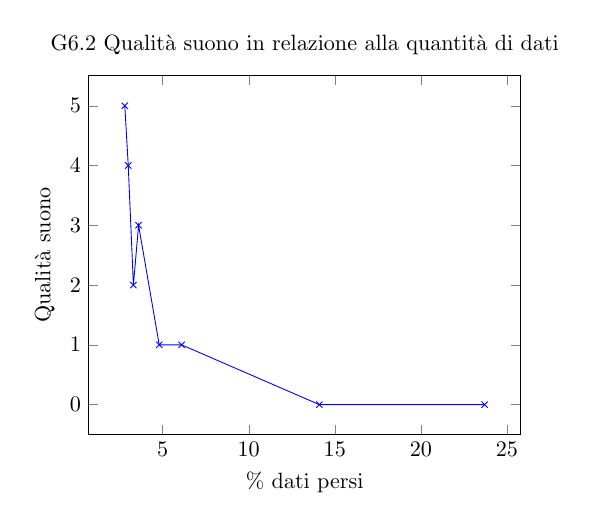
\begin{tikzpicture}[scale=0.8,line width=1pt]
 \begin{axis}[
 ytick={0,1,2,3,4,5},
 %xtick={0,3.84,5.76,11.52,15.36,23.4},
 %xtick={-110},
 %title = bandwidth rapportato al throughput utente nelle varie TM,
 title = G6.2 Qualità suono in relazione alla quantità di dati,
 grid style=dashed,
 xlabel={\% dati persi},
 ylabel={Qualità suono},
 legend style={at={(0.7,0.02)},anchor=south west}
 ]
 %tm1
 \addplot[
 color=blue,
 mark=x]
 table[x=power,y=BER] {
 	power BER
 	2.8 +5
 	3.0 +4
 	3.3 +2
 	3.6 +3
 	4.8 +1
 	6.1 +1
 	14.1 +0
 	23.7 +0
 }; 
 \end{axis}
 \end{tikzpicture}
\end{minipage}
\end{figure}
\begin{figure}
	\centering
	\begin{minipage}[b]{.45\columnwidth}
 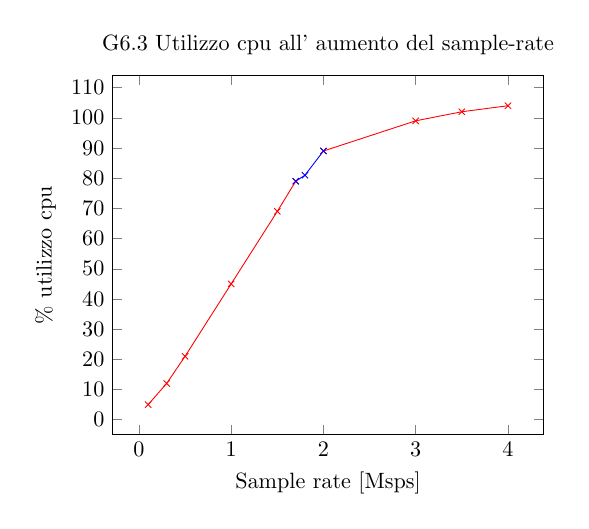
\begin{tikzpicture}[scale=0.8,line width=1pt]
 \begin{axis}[
 ytick={0,10,20,30,40,50,60,70,80,90,100,110},
 %xtick={0,3.84,5.76,11.52,15.36,23.4},
 %xtick={-110},
 %title = bandwidth rapportato al throughput utente nelle varie TM,
 title = G6.3 Utilizzo cpu all' aumento del sample-rate,
 grid style=dashed,
 xlabel={Sample rate [Msps]},
 ylabel={\% utilizzo cpu},
 legend style={at={(0.7,0.02)},anchor=south west}
 ]
 %tm1
 \addplot[
 color=red,
 mark=x]
 table[x=power,y=BER] {
 	power BER
 	0.1 +5
 	0.3 +12
 	0.5 +21
 	1.0 +45
 	1.5 +69
 	1.7 +79
 }; 

\addplot[
color=red,
mark=x]
table[x=power,y=BER] {
	power BER
	2.0 +89
	3.0 +99
	3.5 +102
	4.0 +104
};

\addplot[
color=blue,
mark=x]
table[x=power,y=BER] {
	power BER
	1.7 +79
	1.8 +81
	2.0 +89
}; 

 
 \end{axis}
 \end{tikzpicture}
\end{minipage}
\centering
\begin{minipage}[b]{.45\columnwidth}
 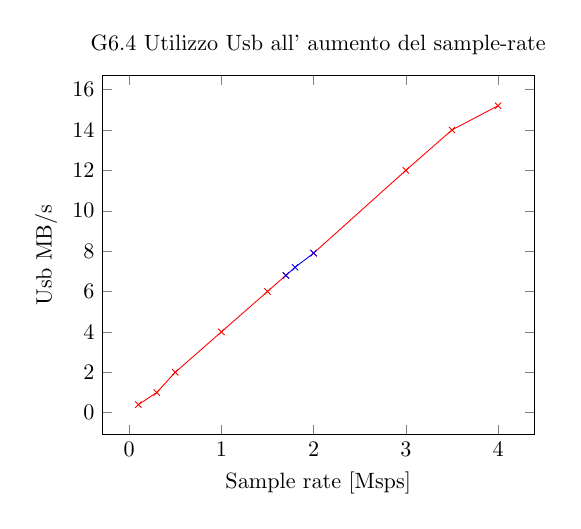
\begin{tikzpicture}[scale=0.8,line width=1pt]
 \begin{axis}[
 ytick={0,2,4,6,8,10,12,14,16},
 %xtick={0,3.84,5.76,11.52,15.36,23.4},
 %xtick={-110},
 %title = bandwidth rapportato al throughput utente nelle varie TM,
 title = G6.4 Utilizzo Usb all' aumento del sample-rate,
 grid style=dashed,
 xlabel={Sample rate [Msps]},
 ylabel={Usb MB/s},
 legend style={at={(0.7,0.02)},anchor=south west}
 ]
 %tm1

\addplot[
color=red,
mark=x]
table[x=power,y=BER] {
	power BER
	0.1 +0.4
	0.3 +1
	0.5 +2
	1.0 +4
	1.5 +6
	1.7 +6.8
};

\addplot[
color=red,
mark=x]
table[x=power,y=BER] {
	power BER
	2.0 +7.9
	3.0 +12
	3.5 +14
	4.0 +15.2
}; 

 \addplot[
color=blue,
mark=x]
table[x=power,y=BER] {
	power BER
	1.7 +6.8
	1.8 +7.2
	2.0 +7.9
}; 

 \end{axis}
 \end{tikzpicture}
\end{minipage}
\end{figure}
 
\begin{figure}[h]
	\centering
	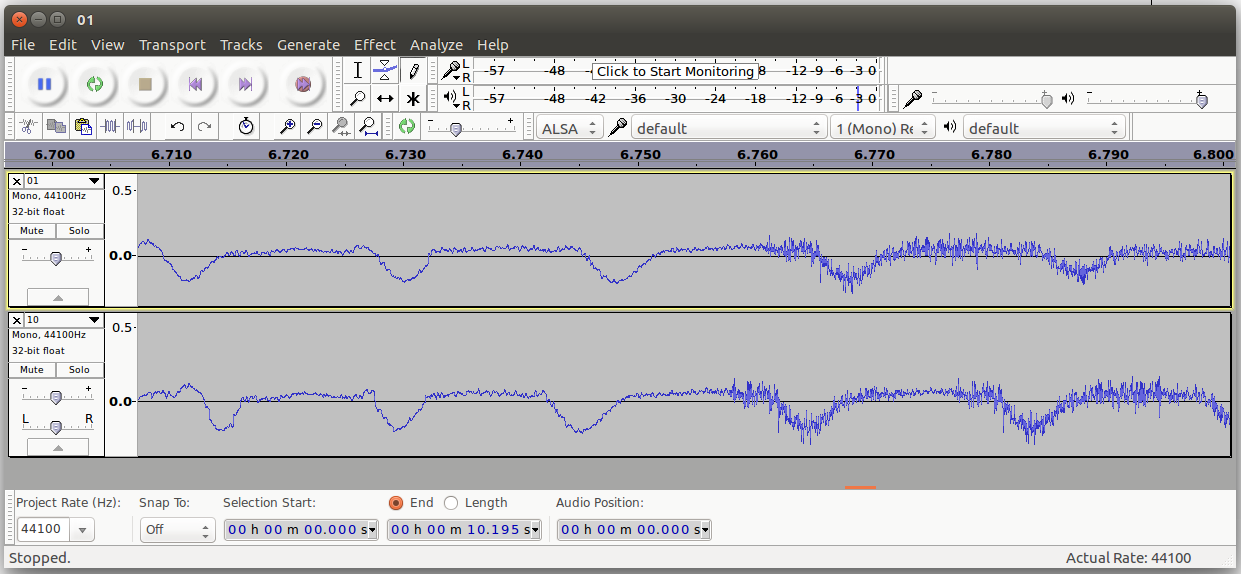
\includegraphics[scale=0.35]{audioRicevuto}
	\caption{Confronto fra l'audio originale e quello ricevuto con perdita del 21\%}
\end{figure}

